\documentclass[
  a4paper,
  oneside,
  BCOR = 10mm,
  DIV = 12,
  12pt,
  headings = normal,
]{scrartcl}

%%% Length calculations
\usepackage{calc}
%%%

%%% Support for color
\usepackage{xcolor}
\definecolor{lightblue}{HTML}{03A9F4}
\definecolor{red}{HTML}{F44336}
%%%

%%% Including graphics
\usepackage{graphicx}
%%%

%%% Font selection
\usepackage{fontspec}

\setromanfont{STIX Two Text}[
  SmallCapsFeatures = {LetterSpace = 8},
]

\setsansfont{IBM Plex Sans}[
  Scale = MatchUppercase,
]

\setmonofont{IBM Plex Mono}[
  Scale = MatchUppercase,
]
%%%

%%% Math typesetting
\usepackage{amsmath}
\usepackage{mathtools}

\usepackage{unicode-math}
\setmathfont{STIX Two Math}

\usepackage{IEEEtrantools}
\usepackage{kbordermatrix}
%%%

%%% List settings
\usepackage{enumitem}
\setlist[enumerate]{
  label*      = {\arabic*.},
  left        = \parindent,
  topsep      = 0\baselineskip,
  parsep      = 0\baselineskip,
  noitemsep, % override itemsep
}
% List settings for levels 2–4
\setlist[enumerate, 2, 3, 4]{
  label*      = {\arabic*.},
  left        = 0em,
  topsep      = 0\baselineskip,
  parsep      = 0\baselineskip,
  noitemsep, % override itemsep
}

\setlist[itemize]{
  label*      = {—},
  left        = \parindent,
  topsep      = 0\baselineskip,
  parsep      = 0\baselineskip,
  itemsep     = 1\baselineskip,
  noitemsep, % override itemsep
}

\setlist[description]{
  font        = {\rmfamily\upshape\bfseries},
  topsep      = 1\baselineskip,
  parsep      = 0\baselineskip,
  itemsep     = 0\baselineskip,
}

%%%

%%% Structural elements typesetting
\setkomafont{pagenumber}{\rmfamily\upshape}
\setkomafont{disposition}{\rmfamily\bfseries}

% Sectioning
\RedeclareSectionCommand[
  beforeskip = -1\baselineskip,
  afterskip  = 1\baselineskip,
  font       = {\normalsize\bfseries\scshape},
]{section}

\RedeclareSectionCommand[
  beforeskip = -1\baselineskip,
  afterskip  = 1\baselineskip,
  font       = {\normalsize\bfseries\itshape},
]{subsection}

\RedeclareSectionCommand[
  beforeskip = -1\baselineskip,
  afterskip  = 1\baselineskip,
  font       = {\normalsize\bfseries},
]{subsubsection}

\RedeclareSectionCommand[
  beforeskip = -1\baselineskip,
  afterskip  = -0.5em,
  font       = {\normalsize\mdseries\scshape\addfontfeatures{Letters = {UppercaseSmallCaps}}},
]{paragraph}
%%%

%%% Typographic enhancements
\usepackage{microtype}
%%%

%%% Language-specific settings
\usepackage{polyglossia}
\setmainlanguage{ukrainian}
\setotherlanguages{english}
%%%

%%% Captions
\usepackage{caption}
\usepackage{subcaption}

%\DeclareCaptionLabelFormat{closing}{#2)}
%\captionsetup[subtable]{labelformat = closing}

%\captionsetup[subfigure]{labelformat = closing}

\captionsetup[table]{
  aboveskip = 0\baselineskip,
  belowskip = 0\baselineskip,
}

\captionsetup[figure]{
  aboveskip = 1\baselineskip,
  belowskip = 0\baselineskip,
}

\captionsetup[subfigure]{
  labelformat = simple,
  labelformat = brace,
  justification = RaggedRight,
  singlelinecheck = false,
}
%%%

%%% Hyphenated ragged typesetting
\usepackage{ragged2e}
%%%

%%% Table typesetting
\usepackage{booktabs}
\usepackage{longtable}

\usepackage{multirow}

\usepackage{array}
\newcolumntype{v}[1]{>{\RaggedRight\arraybackslash\hspace{0pt}}p{#1}}
\newcolumntype{b}[1]{>{\Centering\arraybackslash\hspace{0pt}}p{#1}}
\newcolumntype{n}[1]{>{\RaggedLeft\arraybackslash\hspace{0pt}}p{#1}}
%%%

%%% Drawing
\usepackage{tikz}
\usepackage{tikzscale}
\usetikzlibrary{datavisualization}
\usetikzlibrary{datavisualization.formats.functions}
\usetikzlibrary{positioning}
\usetikzlibrary{patterns}
\usetikzlibrary{intersections}
\usetikzlibrary{arrows.meta} % Stealth arrow tips
\usetikzlibrary{graphs}
\usetikzlibrary{graphdrawing}
\usegdlibrary{layered}
\usetikzlibrary{quotes}

%%%

%%% SI units typesetting
\usepackage{siunitx}
\sisetup{
  output-decimal-marker = {,},
  exponent-product      = {\cdot},
  inter-unit-product    = \ensuremath{{} \cdot {}},
  per-mode              = symbol,
}
%%%

% Code Highlighting
\usepackage{minted}
\setmintedinline{
  style = bw,
  breaklines,
}

\newminted[bashterm]{text}{%
  autogobble,%
  breaklines,%
  style=bw,%
}

\newminted[codegeneric]{text}{%
  autogobble,%
  style=bw,%
  breaklines,%
  fontsize=\small,%
}

\newmintinline{bash}{%
}

\newmintinline[minttext]{text}{%
  breaklines,%
  breakanywhere,%
}

%%% Framing code listings
\usepackage{tcolorbox}
\tcbuselibrary{breakable}
\tcbuselibrary{minted}
\tcbuselibrary{skins}

% Text file listing
\newtcblisting[
  auto counter,
  list inside,
  number within = section,
]{listingplaintext}[3][]{%
  minted language = text,
  minted style    = bw,
  minted options  = {
    autogobble,
    linenos,
    tabsize = 4,
    breaklines,
    breakanywhere,
    fontsize = \footnotesize,
  },
  empty,
  sharp corners,
  coltitle = black,
  borderline horizontal = {1pt}{0pt}{black},
  titlerule = {0.5pt},
  titlerule style = {
    black,
  },
  toptitle = 0.3em,
  bottomtitle = 0.3em,
  before skip      = \intextsep,
  after  skip      = \intextsep,
  title            = {Лістинг \thetcbcounter: #2},
  list entry       = {\protect\numberline{\thetcbcounter}#2},
  left = 0em,
  right = 0em,
  %
  listing only,
  breakable,
  %
  label = {#3},%
}

\newtcbinputlisting[
  use counter from = listingplaintext,
  list inside,
  number within = section
]{\inputplaintext}[4][]{%
  minted language = text,
  minted style    = bw,
  minted options  = {
    autogobble,
    linenos,
    tabsize = 4,
    breaklines,
    breakanywhere,
    fontsize = \footnotesize,
  },
  empty,
  sharp corners,
  coltitle = black,
  borderline horizontal = {1pt}{0pt}{black},
  titlerule = {0.5pt},
  titlerule style = {
    black,
  },
  toptitle = 0.3em,
  bottomtitle = 0.3em,
  before skip      = \intextsep,
  after  skip      = \intextsep,
  title            = {Лістинг \thetcbcounter: #3},
  list entry       = {\protect\numberline{\thetcbcounter}#3},
  left = 0em,
  right = 0em,
  %
  listing file={#2},
  listing only,
  breakable,
  %
  label = {#4}
}

\newtcblisting[
  use counter from = listingplaintext,
  list inside,
  number within = section,
]{listingpython}[3][]{%
  minted language = python,
  minted style    = bw,
  minted options  = {
    autogobble,
    linenos,
    tabsize = 4,
    breaklines,
    breakanywhere,
    fontsize = \footnotesize,
  },
  empty,
  sharp corners,
  coltitle = black,
  borderline horizontal = {1pt}{0pt}{black},
  titlerule = {0.5pt},
  titlerule style = {
    black,
  },
  toptitle = 0.3em,
  bottomtitle = 0.3em,
  before skip      = \intextsep,
  after  skip      = \intextsep,
  title            = {Лістинг \thetcbcounter: #2},
  list entry       = {\protect\numberline{\thetcbcounter}#2},
  left = 0em,
  right = 0em,
  %
  listing only,
  breakable,
  %
  label = {#3},
  %
  #1%
}

\newtcbinputlisting[
  use counter from = listingplaintext,
  list inside,
  number within = section
]{\inputpython}[4][]{%
  minted language = python,
  minted style    = bw,
  minted options  = {
    autogobble,
    linenos,
    tabsize = 4,
    breaklines,
    breakanywhere,
    fontsize = \footnotesize,
  },
  empty,
  sharp corners,
  coltitle = black,
  borderline horizontal = {1pt}{0pt}{black},
  titlerule = {0.5pt},
  titlerule style = {
    black,
  },
  toptitle = 0.3em,
  bottomtitle = 0.3em,
  before skip      = \intextsep,
  after  skip      = \intextsep,
  title            = {Лістинг \thetcbcounter: #3},
  list entry       = {\protect\numberline{\thetcbcounter}#3},
  left = 0em,
  right = 0em,
  %
  listing file={#2},
  listing only,
  breakable,
  %
  label = {#4}
}

% Linux command-line listing
\newtcblisting{linuxterm}%
{%
  % Syntax highlighing options
  listing only,%
  minted language = bash,%
  minted options={%
    autogobble,%
    linenos%
  },%
  % Presentation options
  empty,%
  %% Margins
  sharp corners,%
  toptitle = 0.0em,%
  bottomtitle = 0.0em,%
  left = 0em,%
  right = 0em,%
  before skip = \intextsep,%
  after skip = \intextsep,%
}

\newtcblisting{linuxtermout}%
{%
  % Syntax highlighing options
  listing only,%
  minted language = text,%
  minted options={%
    autogobble,%
    linenos%
  },%
  % Presentation options
  empty,%
  %% Margins
  sharp corners,%
  toptitle = 0.0em,%
  bottomtitle = 0.0em,%
  left = 0em,%
  right = 0em,%
  before skip = \intextsep,%
  after skip = \intextsep,%
}

% Dockerfile listings
\newtcblisting[
  use counter from = listingplaintext,
  list inside,
  number within = section,
]{listingdocker}[3][]{%
  minted language = dockerfile,
  minted style    = bw,
  minted options  = {
    autogobble,%
    linenos,
    tabsize = 4,
    breaklines,
    breakanywhere,
    fontsize = \footnotesize,
  },
  empty,
  sharp corners,
  coltitle = black,
  borderline horizontal = {1pt}{0pt}{black},
  titlerule = {0.5pt},
  titlerule style = {
    black,
  },
  toptitle = 0.3em,
  bottomtitle = 0.3em,
  before skip      = \intextsep,
  after  skip      = \intextsep,
  title            = {Лістинг \thetcbcounter: #2},
  list entry       = {\protect\numberline{\thetcbcounter}#2},
  left = 0em,
  right = 0em,
  %
  listing only,
  breakable,
  %
  label = {#3},%
}

% Docker Compose listings
\newtcblisting[
  use counter from = listingplaintext,
  list inside,
  number within = section,
]{listingdockercompose}[3][]{%
  minted language = yaml,
  minted style    = bw,
  minted options  = {
    autogobble,%
    linenos,
    tabsize = 4,
    breaklines,
    breakanywhere,
    fontsize = \footnotesize,
  },
  empty,
  sharp corners,
  coltitle = black,
  borderline horizontal = {1pt}{0pt}{black},
  titlerule = {0.5pt},
  titlerule style = {
    black,
  },
  toptitle = 0.3em,
  bottomtitle = 0.3em,
  before skip      = \intextsep,
  after  skip      = \intextsep,
  title            = {Лістинг \thetcbcounter: #2},
  list entry       = {\protect\numberline{\thetcbcounter}#2},
  left = 0em,
  right = 0em,
  %
  listing only,
  breakable,
  %
  label = {#3},%
}

% SWI Prolog listings
\newtcblisting[
  use counter from = listingplaintext,
  list inside,
  number within = section,
]{listingprolog}[3][]{%
  minted language = prolog,
  minted style    = bw,
  minted options  = {
    autogobble,%
    linenos,
    tabsize = 4,
    breaklines,
    breakanywhere,
    fontsize = \footnotesize,
  },
  empty,
  sharp corners,
  coltitle = black,
  borderline horizontal = {1pt}{0pt}{black},
  titlerule = {0.5pt},
  titlerule style = {
    black,
  },
  toptitle = 0.3em,
  bottomtitle = 0.3em,
  before skip      = \intextsep,
  after  skip      = \intextsep,
  title            = {Лістинг \thetcbcounter: #2},
  list entry       = {\protect\numberline{\thetcbcounter}#2},
  left = 0em,
  right = 0em,
  %
  listing only,
  breakable,
  %
  label = {#3},%
}

\newtcbinputlisting[
  use counter from = listingplaintext,
  list inside,
  number within = section
]{\inputprolog}[4][]{%
  minted language = prolog,
  minted style    = bw,
  minted options  = {
    autogobble,
    linenos,
    tabsize = 4,
    breaklines,
    breakanywhere,
    fontsize = \footnotesize,
  },
  empty,
  sharp corners,
  coltitle = black,
  borderline horizontal = {1pt}{0pt}{black},
  titlerule = {0.5pt},
  titlerule style = {
    black,
  },
  toptitle = 0.3em,
  bottomtitle = 0.3em,
  before skip      = \intextsep,
  after  skip      = \intextsep,
  title            = {Лістинг \thetcbcounter: #3},
  list entry       = {\protect\numberline{\thetcbcounter}#3},
  left = 0em,
  right = 0em,
  %
  listing file={#2},
  listing only,
  breakable,
  %
  label = {#4}
}


% Customize minted line numbers
\renewcommand{\theFancyVerbLine}{\ttfamily\scriptsize\arabic{FancyVerbLine}}

%%%

%%% Typeset menus and keys
\usepackage{menukeys}[
  os=win,
]
%%%

%%% Links and hyperreferences
\usepackage{hyperref}
\hypersetup{
  bookmarksnumbered = true,
  colorlinks      = false,
  linkbordercolor = red,
  urlbordercolor  = lightblue,
  pdfborderstyle  = {/S/U/W 1.5},
}
%%%

%%% Length adjustment

% Set baselineskip, default is 14.5 pt
\linespread{1.068966} % ~15.5 pt
\setlength{\emergencystretch}{1em}
\setlength{\parindent}{1.5em}
\newlength{\gridunitwidth}
\setlength{\gridunitwidth}{\textwidth / 12}
%%%

%%% Custom commands
\newcommand{\allcaps}[1]{%
  {%
    \addfontfeatures{%
      Letters = UppercaseSmallCaps,
      LetterSpace = 8,%
    }%
    #1%
  }%
}
\newcommand{\filename}[1]{\texttt{#1}}
\newcommand{\progname}[1]{\texttt{#1}}
\newcommand{\commandname}[1]{\texttt{#1}}
\newcommand{\modulename}[1]{\texttt{#1}}
\newcommand{\transeng}[1]{{англ.}~\textit{\textenglish{#1}}}
%%%

%%% Custom math commands
\newcommand{\longvar}[1]{\mathit{#1}}
\newcommand{\vect}[1]{\mathbfit{#1}}
\newcommand{\matr}[1]{\mathbfit{#1}}

\newcommand{\logequiv}{\mathrel{\Longleftrightarrow}} % Logically equivalent

\newcommand{\ssep}{\mid} % set builder separator

\DeclareMathOperator*{\minimize}{min} % minimize for linear programs
\DeclareMathOperator*{\rand}{rand} % rand()

\DeclarePairedDelimiter{\setpower}{\lvert}{\rvert} % set power
%%%

\begin{document}

\begin{titlepage}
    \begin{center}
      Міністерство освіти і~науки України\\
      Національний авіаційний університет\\
      Факультет кібербезпеки, комп'ютерної та~програмної інженерії\\
      Кафедра комп'ютеризованих систем управління

      \vspace{\fill}
        Лабораторна робота №~3.6\\
        з~дисципліни «Технології проектування комп'ютерних систем»\\
        на~тему «Аналіз мереж масового обслуговування»\\
        Варіант №~3

      \vspace{\fill}

      \begin{flushright}
        Виконав:\\
        студент \allcaps{ФККПІ}\\
        групи \allcaps{СП}-425\\
        Клокун В.\,Д.\\
        Перевірила:\\
        Голего Н.\,М.
      \end{flushright}

      Київ 2020
    \end{center}
  \end{titlepage}

  \section{Мета роботи}
    Отримати практичні навички розрахунку системних характеристик експоненціальних мереж масового обслуговування.

  \section{Хід~роботи}
    За варіантом завдання дана експоненціальна~МеМО. Відповідно до завдання варіанта~(табл.~\ref{tab:task}), побудуємо її модифіковану схему~(рис.~\ref{fig:schematic}).

    \begin{table}[!htbp]
      \centering
      \caption{Завдання варіанта}
      \label{tab:task}
      \newlength{\smocolwidth}
      \setlength{\smocolwidth}{9 \gridunitwidth / 6}
      \begin{tabular}{
        v{3\gridunitwidth - 2\tabcolsep}
        *{6}{n{1\smocolwidth - 2\tabcolsep}}
      }
        \toprule
                         & \multicolumn{6}{c}{Номера~\allcaps{СМО}}\\
                         \cmidrule(lr){2-7}
          Номер варіанту & 1 & 2 & 3 & 4 & 5 & 6 \\
        \midrule
          3              & − & − & + & + & − & + \\
        \bottomrule
      \end{tabular}
    \end{table}

    \begin{figure}[!htbp]
      \centering
      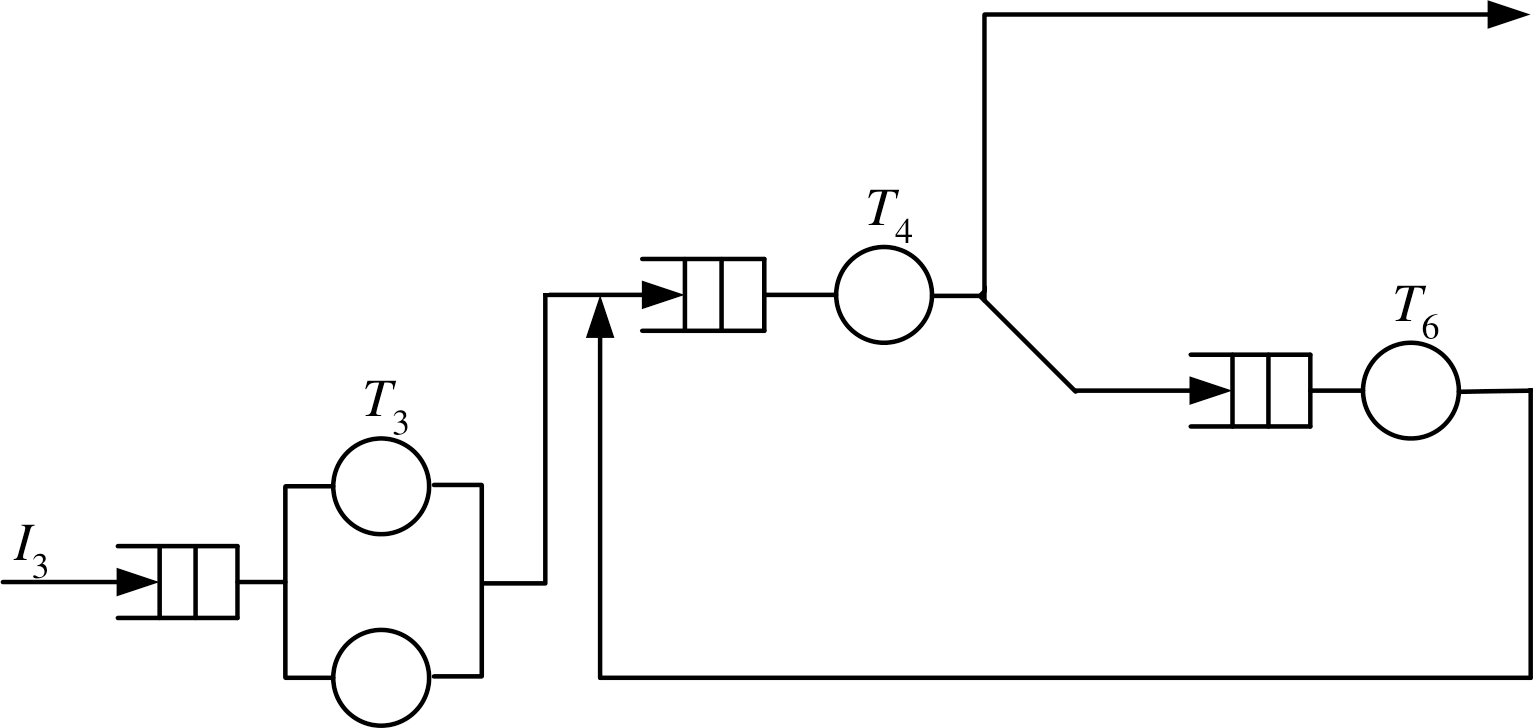
\includegraphics[width = 9 \gridunitwidth]{./assets/01-reduced-schematic.png}
      \caption{Модифікована схема, яка відповідає завданню варіанта}
      \label{fig:schematic}
    \end{figure}

    Враховуючи зміни, внесені до схеми, наведемо параметри заданої системи масового обслуговування:
    \begin{enumerate}
      \item Число систем масового обслуговування~$N = 3$.
      \item Число каналів~$K$ в системі масового обслуговування: $K_3 = 2, K_4 = 1, K_6 = 1$.
      \item Ймовірності переходів~$p_{ij}$: $p_{34} = 1$; $p_{40} = \num{0.8}$, так як зі схеми була видалена система №~5; $p_{46} = \num{0.2}$; $p_{61} = 1$. Тоді матриця переходів виглядає так:
        \begin{IEEEeqnarray*}{rCl}
          P = \kbordermatrix{
              & 0   & 3 & 4 & 6 \\
            3 & 0   & 0 & 1 & 0 \\
            4 & \num{0.8} & 0 & 0 & \num{0.2} \\
            6 & 0   & 0 & 1 & 0 \\
          }
        \end{IEEEeqnarray*}
      \item Інтенсивності вхідних потоків заявок~$I_{1} = 0$, $I_2 = 0$, $I_3 = 1/50$.
      \item Середні часи обслуговування: $T_3 = 90$, $T_4 = 7$, $T_6 = 40$.
    \end{enumerate}

    \subsection{Баланс інтенсивностей}
      За наявними завданнями складаємо рівняння балансу інтенсивностей, перетворюємо та спрощуємо їх, щоб знайти інтенсивності~$\lambda_n$:
      \begin{IEEEeqnarray*}{rCl}
        \left\{
          \begin{IEEEeqnarraybox}[
            \IEEEeqnarraystrutmode
            \IEEEeqnarraystrutsizeadd{2pt}{2pt}
          ][c]{rCl}
            \lambda_3 &=& I_3 \\
            \lambda_4 &=& \lambda_3 + \lambda_6 \\
            \lambda_6 &=& p_{46} \lambda_4
          \end{IEEEeqnarraybox}
        \right.
        &\implies&
        \left\{
          \begin{IEEEeqnarraybox}[
            \IEEEeqnarraystrutmode
            \IEEEeqnarraystrutsizeadd{2pt}{2pt}
          ][c]{rCl}
            \lambda_3 &=& \frac{1}{50} = \num{0.02} \\
            \lambda_4 &=& \num{0.02} + p_{46} \lambda_4 \\
            \lambda_6 &=& p_{46} \lambda_4 = \num{0.2} \lambda_4
          \end{IEEEeqnarraybox}
        \right.
        \implies
        \left\{
          \begin{IEEEeqnarraybox}[
            \IEEEeqnarraystrutmode
            \IEEEeqnarraystrutsizeadd{2pt}{2pt}
          ][c]{rCl}
            \lambda_3 &=& \num{0.02} \\
            \lambda_4 &=& \num{0.02} + \num{0.2} \lambda_4 \\
            \lambda_6 &=& \num{0.2} \lambda_4
          \end{IEEEeqnarraybox}
        \right.
        \\[2\jot]
        & \implies &
        \left\{
          \begin{IEEEeqnarraybox}[
            \IEEEeqnarraystrutmode
            \IEEEeqnarraystrutsizeadd{2pt}{2pt}
          ][c]{l}
            \lambda_3 = \num{0.02} \\
            \num{0.8} \lambda_4 = \num{0.02} \\
            \lambda_6 = \num{0.2} \lambda_4
          \end{IEEEeqnarraybox}
        \right.
        \implies
        \left\{
          \begin{IEEEeqnarraybox}[
            \IEEEeqnarraystrutmode
            \IEEEeqnarraystrutsizeadd{2pt}{2pt}
          ][c]{l}
            \lambda_3 = \num{0.02} \\
            \lambda_4 = \num{0.02} : \num{0.8} = \num{0.025} \\
            \lambda_6 = \num{0.2} \cdot \num{0.025} = \num{0.005}
          \end{IEEEeqnarraybox}
        \right.
      \end{IEEEeqnarray*}
      Отже, отримали: $\lambda_3 = \num{0.02}$, $\lambda_4 = \num{0.025}$, $\lambda_6 = \num{0.005}$.

    \subsection{Середній час перебування заявки в~МеМО}
      \label{ssec:avg-time}
      Щоб знайти середній час перебування заявки в~МеМО, необхідно обчислити значення середнього числа заявок в каналі~$\rho_i$ для кожної системи масового обслуговування:
      \begin{IEEEeqnarray*}{rCl}
        \rho_3 &=& \lambda_3 \cdot \overline{T}_{\text{обсл}_3} / 2 = \num{0.02} \cdot 90 / 2 = \num{0.9},\\
        \rho_4 &=& \lambda_4 \cdot \overline{T}_{\text{обсл}_4} = \num{0.025} \cdot 7 = \num{0.175},\\
        \rho_6 &=& \lambda_6 \cdot \overline{T}_{\text{обсл}_6} = \num{0.05} \cdot 40 = \num{0.2}.
      \end{IEEEeqnarray*}

      Обчисливши значення сердніх чисел заявок в каналах, можемо обчислити середній час перебування заявки в кожному каналі~$\overline{T}_{\text{пер}_i}$ за формулою:
      \begin{IEEEeqnarray*}{rCl}
        \overline{T}_{\text{пер}_i}
        = \frac{\overline{T}_{\text{обсл}_i} \rho_i}{1 - \rho_i}.
      \end{IEEEeqnarray*}
      Обчислюємо за отриманими даними:
      \begin{IEEEeqnarray*}{rCl}
        \overline{T}_{\text{пер}_3}
        &=& \frac{\overline{T}_{\text{обсл}_3} \cdot \rho_3}{1 - \rho_3}
        = \frac{90 \cdot \num{0.9}}{1 - \num{0.9}}
        = 810,
        \quad
        \overline{T}_{\text{пер}_4}
        = \frac{\overline{T}_{\text{обсл}_4} \cdot \rho_4}{1 - \rho_4}
        = \frac{7 \cdot \num{0.175}}{1 - \num{0.175}}
        = \num{1.48},
        \\
        \overline{T}_{\text{пер}_6}
        &=& \frac{\overline{T}_{\text{обсл}_6} \cdot \rho_6}{1 - \rho_6}
        = \frac{40 \cdot \num{0.2}}{1 - \num{0.2}}
        = 10.
      \end{IEEEeqnarray*}
      За середніми значення для кожного каналу, можна обчислити середнє значення для мережі за формулою:
      \begin{IEEEeqnarray*}{rCl}
        \overline{T}_{\text{пер}} = \frac{1}{I} \sum_{j=1}^{N} \lambda_j \overline{T}_{\text{пер}_j}.
      \end{IEEEeqnarray*}
      Обчислюємо середнє значення для заданої мережі.
      \begin{IEEEeqnarray*}{rCl}
        \overline{T}_{\text{пер}}
        &=& \frac{1}{I} \sum_{j=1}^{N} \lambda_j \overline{T}_{\text{пер}_j}
        = \frac{1}{\num{0.02}} \left(
          \lambda_3 \overline{T}_{\text{пер}_3}
          + \lambda_4 \overline{T}_{\text{пер}_4}
          + \lambda_6 \overline{T}_{\text{пер}_6}
        \right)
        \\
        &=& 50 \cdot (\num{0.02} + 810 + \num{0.025} \cdot \num{1.48} + \num{0.005} \cdot 10)
        = \num{814.35}.
      \end{IEEEeqnarray*}
      Отже, середній час перебування заявки у мережі складає~$\overline{T}_{\text{пер}} = \num{814.35}$.

    \subsection{Передаточні коефіцієнти}
      Щоб визначити передаточні коефіцієнти~$\alpha_{ij}$, необхідно скласти рівняння балансу, враховуючи всі вхідні потоки~$I_i$:
      \begin{IEEEeqnarray*}{rCl}
        \left\{
        \begin{IEEEeqnarraybox}[
            \IEEEeqnarraystrutmode
            \IEEEeqnarraystrutsizeadd{2pt}{2pt}
        ][c]{l}
          \lambda_3 = I_3 \\
          \lambda_4 = \lambda_3 + \lambda_6 + I_4 \\
          \lambda_6 = p_{46} + I_6
        \end{IEEEeqnarraybox}
        \right.
        &\implies&
        \left\{
        \begin{IEEEeqnarraybox}[
            \IEEEeqnarraystrutmode
            \IEEEeqnarraystrutsizeadd{2pt}{2pt}
        ][c]{l}
          \lambda_3 = I_3 \\
          \lambda_4 = I_3 + (\num{0.2} \lambda_4 + I_6) + I_4 \\
          \lambda_6 = \num{0.2} \lambda_4 + I_6
        \end{IEEEeqnarraybox}
        \right.
        \implies
        \left\{
        \begin{IEEEeqnarraybox}[
            \IEEEeqnarraystrutmode
            \IEEEeqnarraystrutsizeadd{2pt}{2pt}
        ][c]{l}
          \lambda_3 = I_3 \\
          \num{0.8} \lambda_4 = I_3 + I_4 + I_6 \\
          \lambda_6 = \num{0.2} \lambda_4 + I_6
        \end{IEEEeqnarraybox}
        \right.
        \\
        &\implies&
        \left\{
        \begin{IEEEeqnarraybox}[
            \IEEEeqnarraystrutmode
            \IEEEeqnarraystrutsizeadd{2pt}{2pt}
        ][c]{l}
          \lambda_3 = I_3 \\
          \lambda_4 = \frac{I_3 + I_4 + I_6}{\num{0.8}} \\[2\jot]
          \lambda_6 = \frac{\num{0.2} (I_3 + I_4 + I_6) }{\num{0.8}} + I_6
        \end{IEEEeqnarraybox}
        \right.
        \implies
        \left\{
        \begin{IEEEeqnarraybox}[
            \IEEEeqnarraystrutmode
            \IEEEeqnarraystrutsizeadd{2pt}{2pt}
        ][c]{l}
          \lambda_3 = I_3 \\
          \lambda_4 = \num{1.25} (I_3 + I_4 + I_6) \\
          \lambda_6 = \frac{I_3 + I_4 + I_6}{4} + I_6
        \end{IEEEeqnarraybox}
        \right.
      \end{IEEEeqnarray*}
      Щоб знайти передаточні коефіцієнти, підставляємо кортежі значень інтенсивностей потоків~$(I_3, I_4, I_6)$, де~$I_i = 1, I_{j \in \{ N \setminus j \} } = 0$ і отримаємо:
      \begin{IEEEeqnarray*}{l}
        \begin{IEEEeqnarraybox}[
            \IEEEeqnarraystrutmode
            \IEEEeqnarraystrutsizeadd{2pt}{2pt}
        ][c]{l.rCl}
          I = (1, 0, 0){:} & \lambda_i &=& (1; \num{1.25}; \num{0.25}),\\
          I = (0, 1, 0){:} & \lambda_i &=& (0; \num{1.25}; \num{0.25}),\\
          I = (0, 0, 1){:} & \lambda_i &=& (0; \num{1.25}; \num{1.25}).
        \end{IEEEeqnarraybox}
      \end{IEEEeqnarray*}
      Отже, матриця передаточних коефіцієнтів~$A$:
      \begin{IEEEeqnarray*}{l}
        \mathbf{A} =
        \begin{bmatrix}
          1 & \num{1.25} & \num{0.25} \\
          0 & \num{1.25} & \num{0.25} \\
          0 & \num{1.25} & \num{1.25}
        \end{bmatrix}
      \end{IEEEeqnarray*}

    \subsection{Розрахунок вхідних середніх проміжків часу перебування в мережі~$F_1, \dots, F_N$}
     Щоб обчислити вхідні середні проміжки часу перебування в мережі~$F_1, \dots, F_N$, достатньо помножити передаточні коефіцієнти на середній час перебування заявок. Тоді отримаємо:
     \begin{IEEEeqnarray*}{rCl}
       \mathbf{A} \cdot \begin{bmatrix}
         \overline{T}_{\text{пер}_3} &
         \overline{T}_{\text{пер}_4} &
         \overline{T}_{\text{пер}_6}
       \end{bmatrix}^T
       =
       \mathbf{A}
       \cdot
       \begin{bmatrix} 810 & \num{1.48} & 10\end{bmatrix}^T
       =
       \begin{bmatrix} \num{814.35} & \num{4.35} & \num{14.35} \end{bmatrix}^T.
     \end{IEEEeqnarray*}

     Щоб перевірити дані, наприклад, для першого вхідного потоку, необхідно скласти формулу для заданої схеми:
     \begin{IEEEeqnarray*}{l}
       \left\{
        \begin{IEEEeqnarraybox}[
            \IEEEeqnarraystrutmode
            \IEEEeqnarraystrutsizeadd{2pt}{2pt}
        ][c]{rCl}
          F_3 &=& \overline{T}_{\text{пер}_3} + F_4 \\
          F_4 &=& \overline{T}_{\text{пер}_4} + \num{0.2} F_6 \\
          F_6 &=& \overline{T}_{\text{пер}_6} + F_4.
        \end{IEEEeqnarraybox}
        \right.
        \implies
       \left\{
        \begin{IEEEeqnarraybox}[
            \IEEEeqnarraystrutmode
            \IEEEeqnarraystrutsizeadd{2pt}{2pt}
        ][c]{rCl}
          F_3 &=& 810 + F_4 \\
          F_4 &=& \num{1.48} + \num{0.2} F_6 \\
          F_6 &=& 10 + F_4.
        \end{IEEEeqnarraybox}
        \right.
        \implies
       \left\{
        \begin{IEEEeqnarraybox}[
            \IEEEeqnarraystrutmode
            \IEEEeqnarraystrutsizeadd{2pt}{2pt}
        ][c]{rCl}
          F_3 &=& \num{814.35} \\
          F_4 &=& \num{4.35} \\
          F_6 &=& \num{14.35}.
        \end{IEEEeqnarraybox}
        \right.
     \end{IEEEeqnarray*}
     Дані збігаються, отже розрахунки виконані вірно: $F_3 = \num{814.35}$, $F_4 = \num{4.35}$, $F_6 = \num{14.35}$.

    \subsection{Розрахунок часу перебування в МеМО~$\overline{T}_{\text{пер}}$ та для кожної~\allcaps{СМО}~$\overline{T}_{\text{пер}_i}$}
      Розрахунки наведені в підрозділі~\ref{ssec:avg-time}.

  \section{Висновок}
    Виконуючи дану лабораторну роботу, ми отримали практичні навички розрахунку системних характеристик експоненціальних мереж масового обслуговування.

\end{document}
